\section{Ejercicios Denavit Hartenberg}
\vspace{10mm}

\textbf{Ejercicio 2:}
\vspace{5mm}

\begin{figure}[htbp]
	\centering
	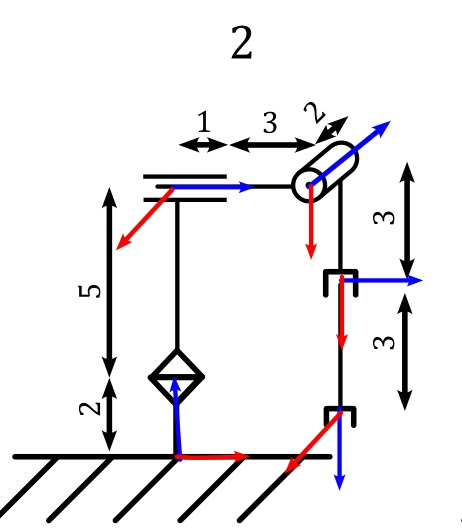
\includegraphics[width=0.5\linewidth]{img/2EJ}
	\caption{Diagrama del ejercicio 2.}
	\label{fig:2ej}
\end{figure}

\begin{figure}[htbp]
	\centering
	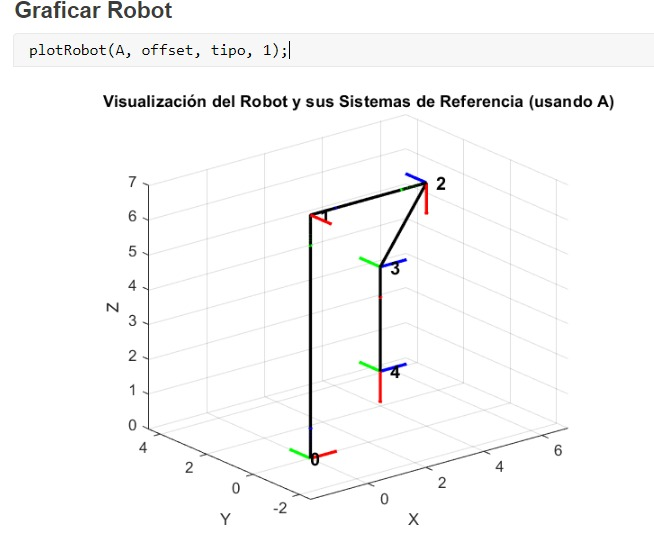
\includegraphics[width=0.5\linewidth]{img/EJ2}
	\caption{Diagrama de MATLAB.}
	\label{fig:ej2}
\end{figure}

\clearpage % Fuerza el cambio de página antes del siguiente ejercicio

\textbf{Ejercicio 3:}
\vspace{5mm}

\begin{figure}[htbp]
	\centering
	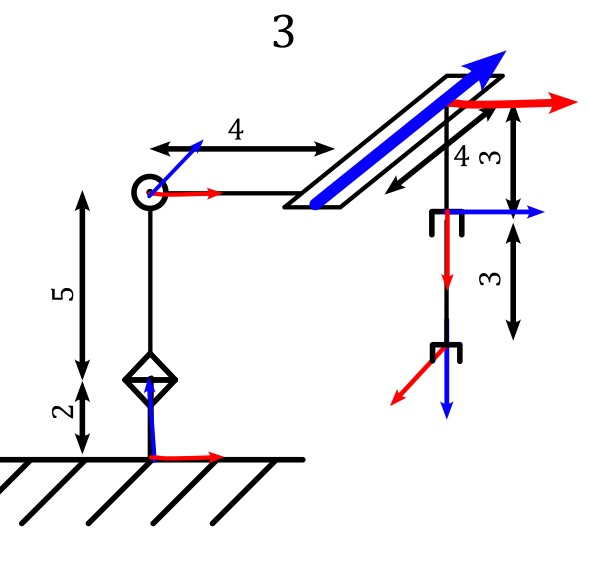
\includegraphics[width=0.5\linewidth]{img/3EJ}
	\caption{Diagrama del ejercicio 3.}
	\label{fig:3ej}
\end{figure}

\begin{figure}[htbp]
	\centering
	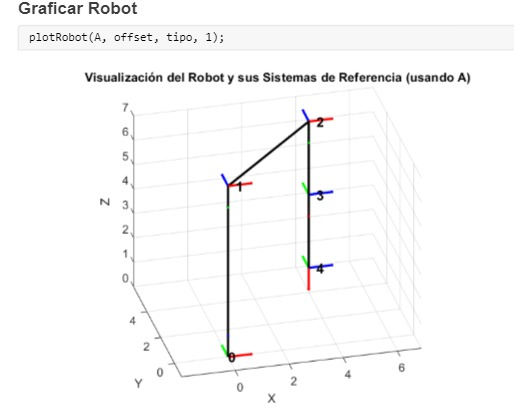
\includegraphics[width=0.5\linewidth]{img/EJ3}
	\caption{Diagrama de MATLAB.}
	\label{fig:ej3}
\end{figure}

\clearpage

\textbf{Ejercicio 4:}
\vspace{5mm}

\begin{figure}[htbp]
	\centering
	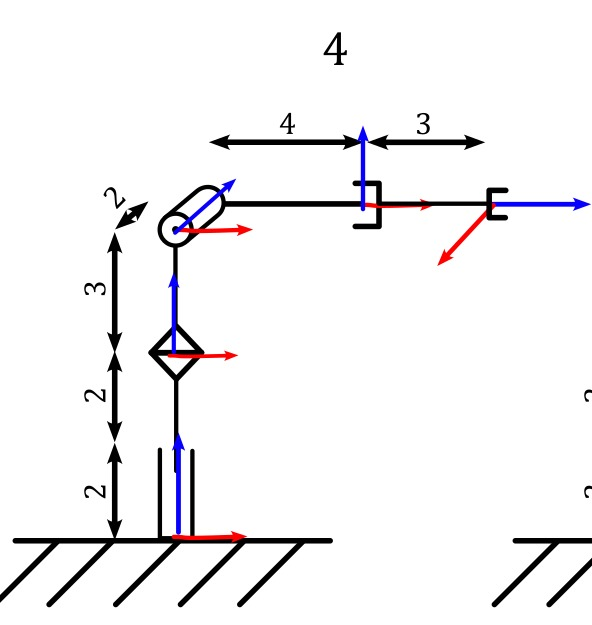
\includegraphics[width=0.5\linewidth]{img/4EJ}
	\caption{Diagrama del ejercicio 4.}
	\label{fig:4ej}
\end{figure}

\begin{figure}[htbp]
	\centering
	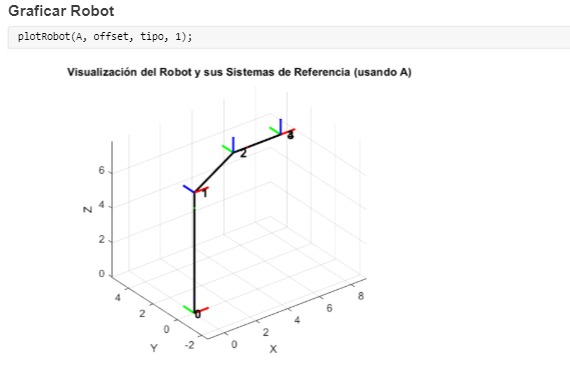
\includegraphics[width=0.5\linewidth]{img/EJ4}
	\caption{Diagrama de MATLAB.}
	\label{fig:ej4}
\end{figure}

\clearpage

\textbf{Ejercicio 9:}
\vspace{5mm}

\begin{figure}[htbp]
	\centering
	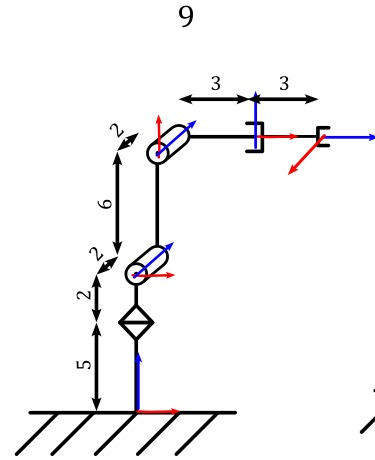
\includegraphics[width=0.5\linewidth]{img/9EJ}
	\caption{Diagrama del ejercicio 9.}
	\label{fig:9ej}
\end{figure}

\begin{figure}[htbp]
	\centering
	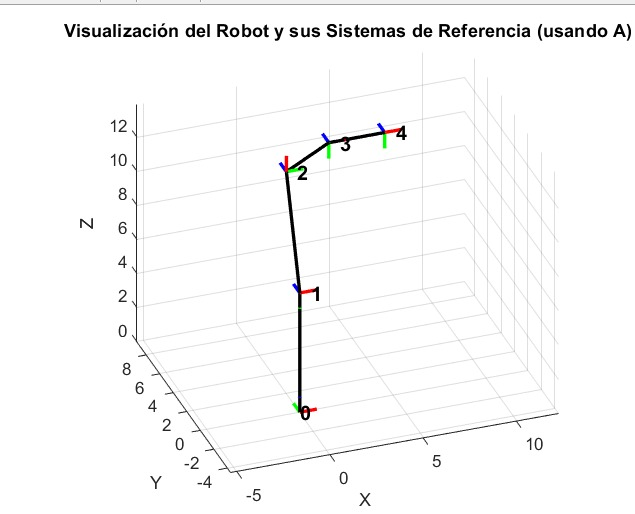
\includegraphics[width=0.5\linewidth]{img/EJ9}
	\caption{Diagrama de MATLAB.}
	\label{fig:ej9}
\end{figure}

\clearpage

\textbf{Ejercicio 10:}
\vspace{5mm}

\begin{figure}[htbp]
	\centering
	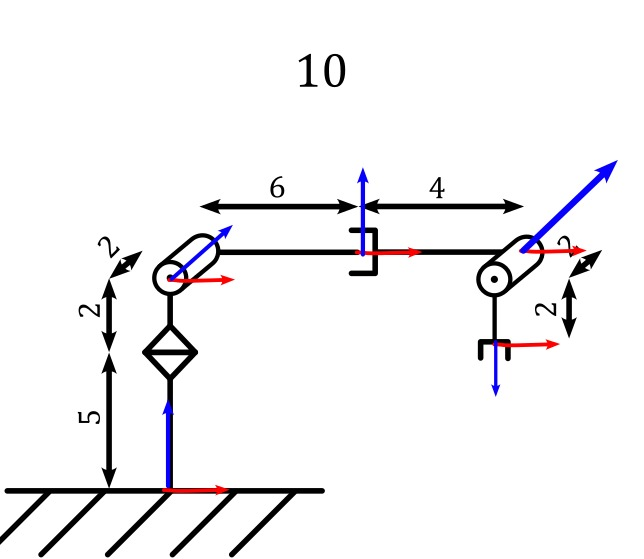
\includegraphics[width=0.5\linewidth]{img/10ej}
	\caption{Diagrama del ejercicio 10.}
	\label{fig:10ej}
\end{figure}

\begin{figure}[htbp]
	\centering
	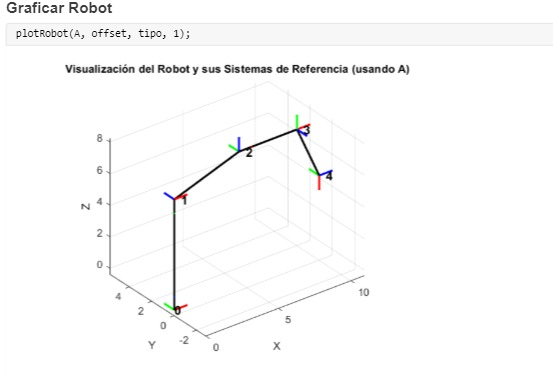
\includegraphics[width=0.5\linewidth]{img/EJ10}
	\caption{Diagrama de MATLAB.}
	\label{fig:ej10}
\end{figure}

\clearpage
